\newcommand{\cmark}{\ding{51}}%
\newcommand{\xmark}{\ding{55}}%
\section{Analysis}

In this section, we analyze how \POWSM works, focusing on the phonetic-aware encoder and task- and language-specific tokens, which are the defining features of the model.

\subsection{Behavior of the speech encoder}

\paragraph{The CTC encoder prefers fine-grained phones without suprasegmentals}
\label{sec:analysis-ctc-target}
We observed that mixing phones and orthography as encoder targets hindered training, because the same speech input would have different encoder CTC targets for different tasks. 
Therefore, we used phones as encoder targets, encouraging general representations of sounds to be shared across languages.

To determine the most effective unit for the CTC encoder, we fix the decoder vocabulary to PanPhon phones and compared four encoder targets: (1) Unicode code points vs. PanPhon, and (2) sequences with vs. without suprasegmentals (length and break marks). Unicode code points offer simplicity and a smaller vocabulary but split phones into unnatural units (e.g. \textipa{/p\super{h}/}) and increase sequence length, while PanPhon represents each phone-diacritic combination as a unit (e.g. \textipa{/p\super{h}/}), yielding a more natural monotonic sequence at the expense of sparsity and potential out-of-vocabulary issues. Suprasegmentals such as \textipa{/\textlengthmark/}, though phonemic in many languages, confuse PR models \citep{zhu-etal-2025-zipa}. 


We run small-scale experiments on a 1k-hour subset of the multi-task data (250 hours of speech repeated across four tasks).
We use the validation CER of the encoder-CTC output as a proxy for training efficiency. 
An earlier drop indicates that the encoder is learning a useful alignment early, which improves representations fed into the decoder and accelerates overall convergence. 
% fast is ambiguous (could also mean steep convergence)
In \autoref{fig:ctc-vocab}, PanPhon tokenization without suprasegmentals shows the earliest drop, suggesting that alignment with decoder units aids training, while
collapsing suprasegmental distinctions for CTC reduces confusion.

\begin{figure}[t]
    \centering
    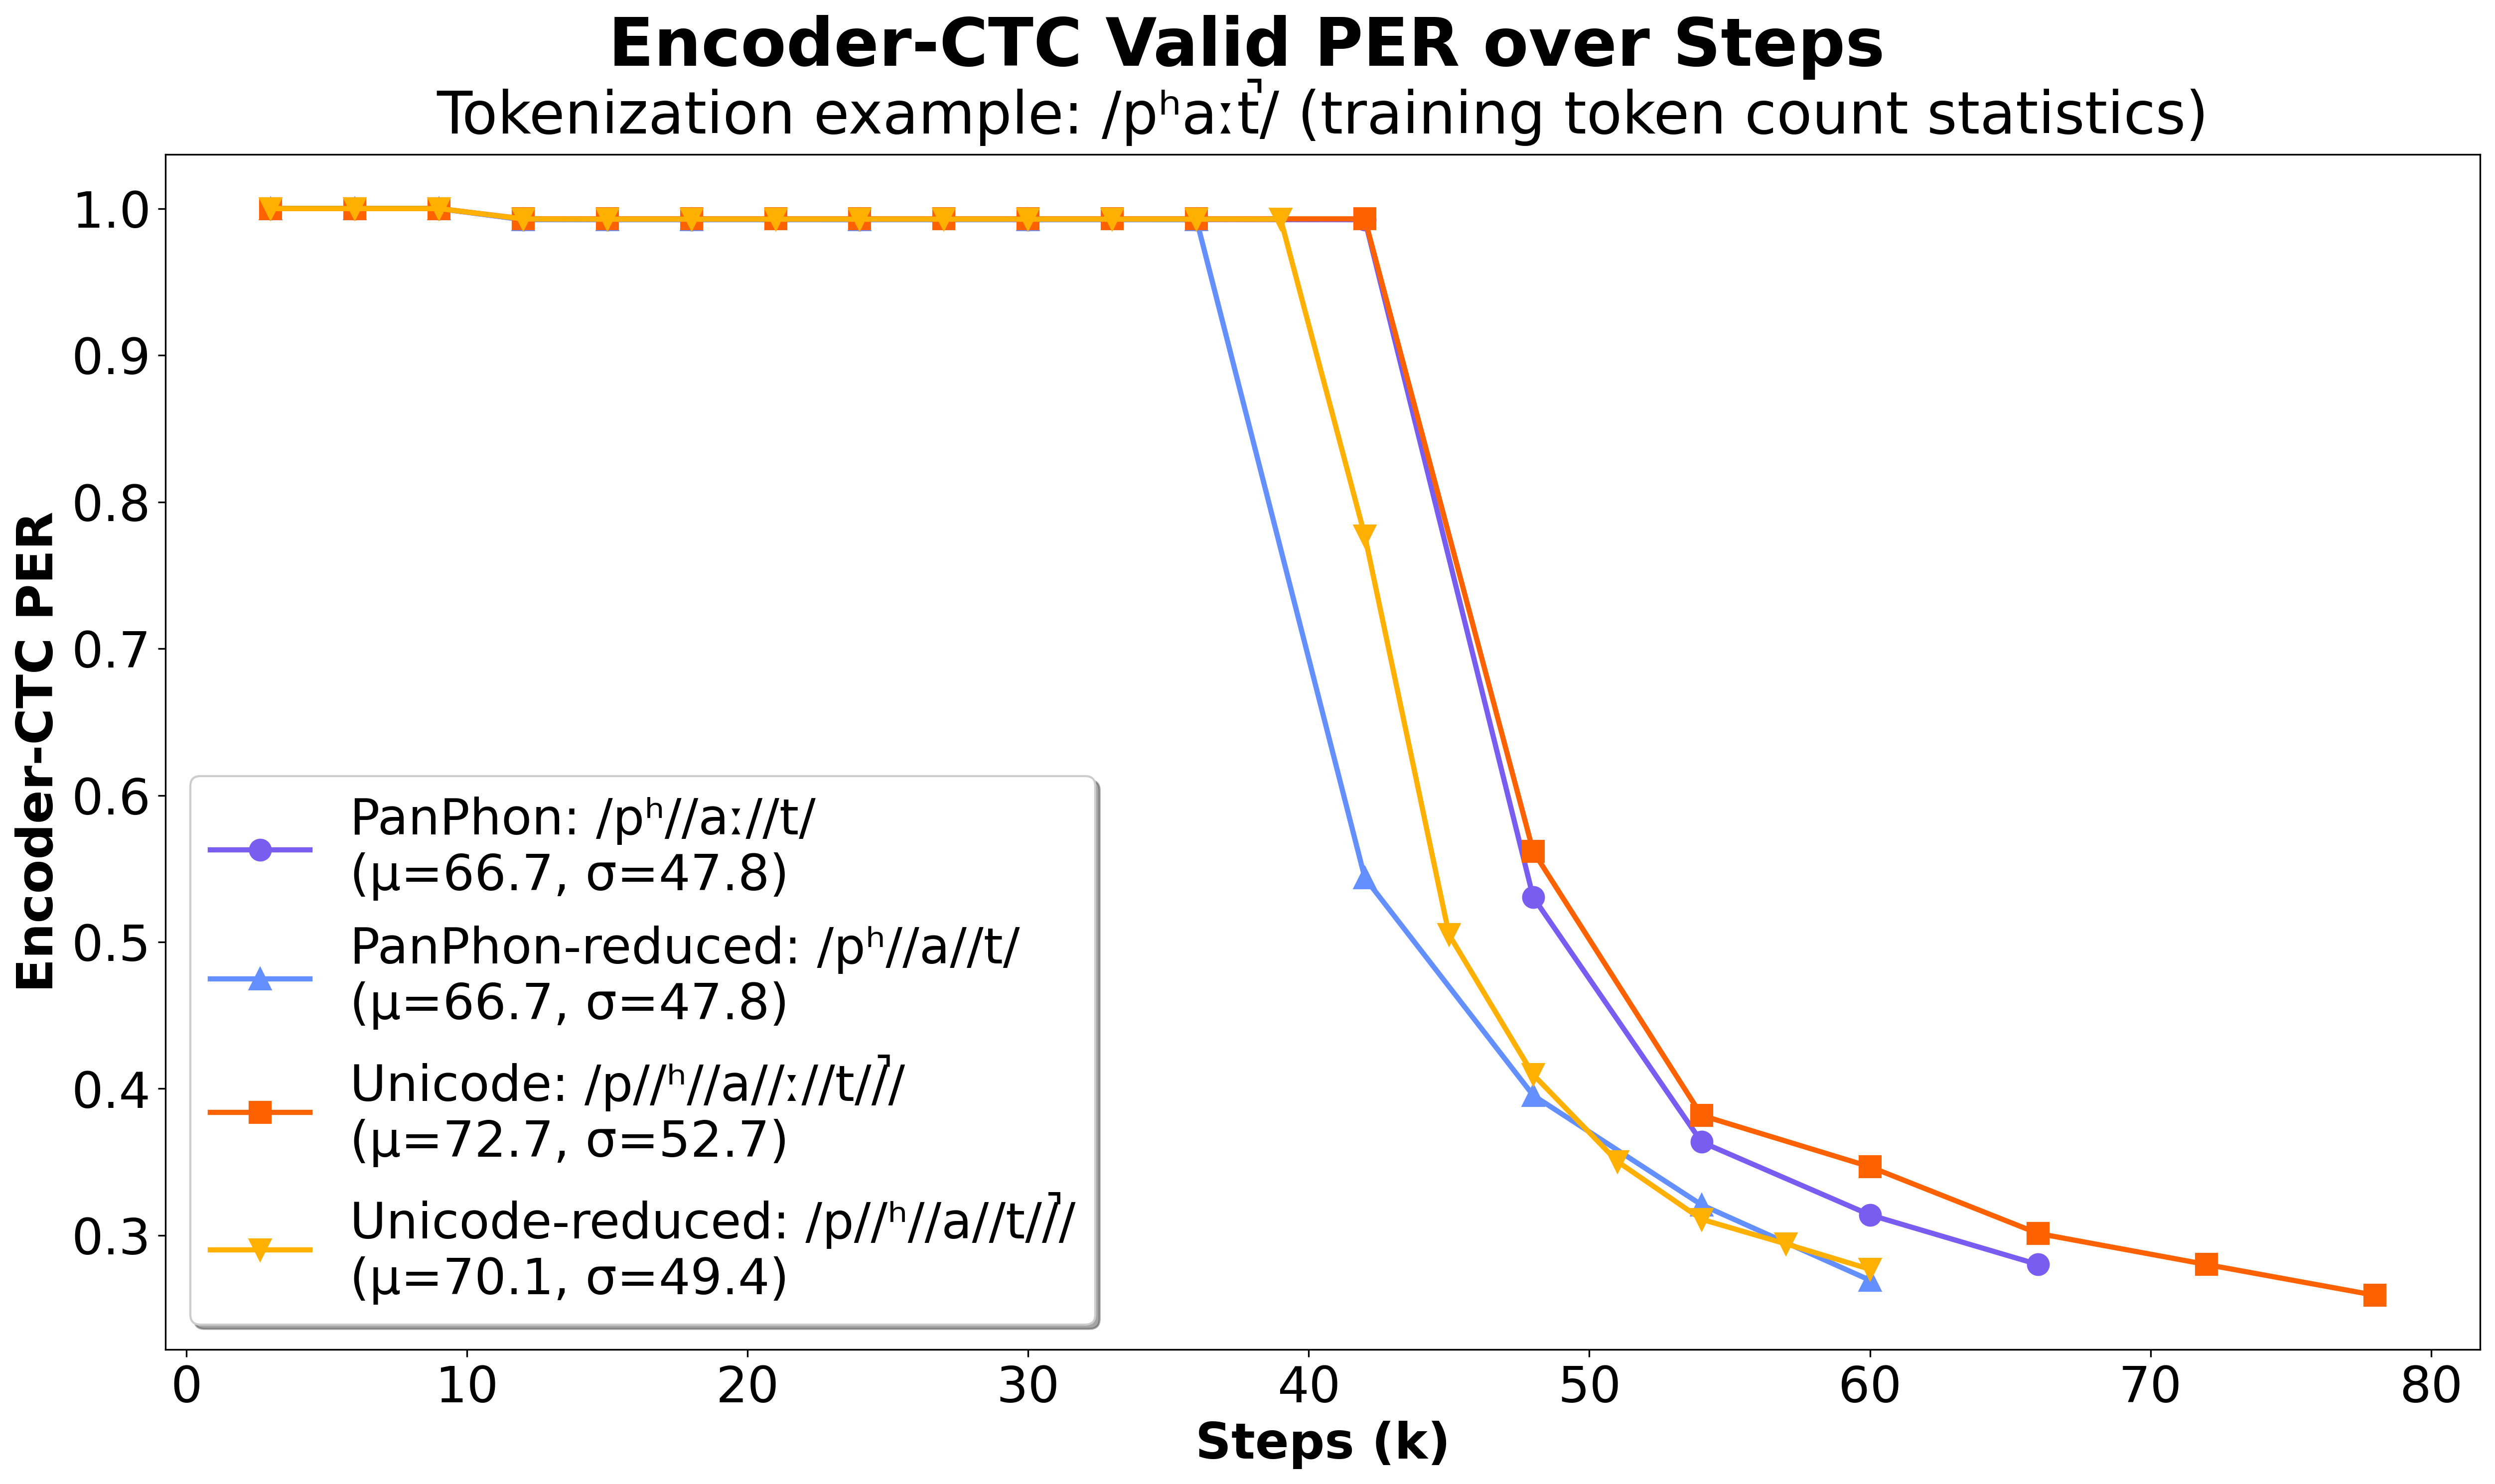
\includegraphics[width=\linewidth]{figures/encctc_target.png}
    \caption{Validation PER of encoder-CTC during training. Removing suprasegmentals from the training target of encoder accelerates convergence.
    % Fixed: \reviewer{Please enlarge Figure 2 and improve its readability (font size, caption clarity).}
    }
    \label{fig:ctc-vocab}
\end{figure}


\paragraph{Increased encoder weights benefit PR on out-of-domain data}
\label{sec:analysis-ctc-weight}
As in other encoder-decoder models \cite{gong23d_interspeech,  radford2023robust}, we expect the encoder of \POWSM to capture more general acoustic patterns, while the decoder handles language and task-specific output formats. Therefore, 
% instead of ignoring the encoder output as in most S2T tasks, 
we investigate whether emphasizing the encoder more during different stages of model development affects performance.
To balance data diversity with inference compute costs, we selected two smaller datasets from each category with distinct characteristics.

As shown in \autoref{tab:ctc-weight}, higher CTC decoding weights improve PR performance on out-of-domain data but degrade it on in-domain data, as expected.
This echoes \citet{zhu-etal-2025-zipa}'s finding that RNN-T \citep{graves2014towards}, an encoder-only speech-to-text model with an autoregressive text prediction network, hurts generalization to unseen patterns of phones.
% Jian: ``learning the causal dependencies between phones can also hurt the multilingual generalizability, as unseen languages might have a different phonological structure''
We hypothesize that the decoder is performing implicit phonotactic language modeling and ``smooths'' phonetic variation towards more probabilistically likely phone patterns, as \citet{zhu-etal-2025-zipa} described.

Next, we examine whether focusing more on the CTC loss through training widens this gap in performance between in-domain and out-of-domain data.
We find that fine-tuning with a higher CTC loss weight $\alpha_\text{ctc}$ after convergence does not improve out-of-domain performance and can even degrade it. Randomly varying $\alpha_\text{ctc}$ for each batch also shows no improvement.
In contrast, training with a higher $\alpha_\text{ctc}$ from the start benefits the out-of-domain distribution, achieving the lowest PFER on unseen languages with greedy decoding, while the PFER on in-domain data is comparatively higher.
These results suggest that assigning a higher weight to the encoder during training and inference improves PR, highlighting a common trade-off between in-domain performance and generalization.




\begin{table}[h]
\vspace{-2mm}
\centering
\small
\setlength{\tabcolsep}{4pt} % Adjust column spacing
\renewcommand{\arraystretch}{1.2}
\resizebox{\columnwidth}{!}{
\begin{tabular}{l cc| cccc}
\toprule
& \multicolumn{2}{c}{In-domain} & \multicolumn{4}{c}{Out-of-domain}\\
Setup & \texttt{ita} & \texttt{ pol } & VoxA. & Tusom. & DRC-SE & EpaDB\\
\midrule
\multicolumn{3}{l|}{\textbf{Decoding}}\\
\texttt{ctc=0.3} & \textbf{1.66} & \textbf{1.36} & \textbf{17.58} & 33.52 & 18.21 & 11.88\\
\texttt{ctc=0.7} & 1.97 & 1.37 & 17.92 & 24.29 & 18.05 & 11.82\\
\texttt{ctc=0.9} &2.05 & 1.38 & 19.27 & \textbf{22.94} & \textbf{17.67} & \textbf{11.80}\\
\multicolumn{3}{l|}{\textbf{Pre-training / Fine-tuning}}\\
$\alpha_\text{ctc}$=0.3 & \textbf{1.81} & 1.60 & 16.02 & 22.47 & 18.59 & 11.66\\
$\rightarrow$ Ft, $\alpha_\text{ctc}$=0.5& 1.94 & \textbf{1.53} & 17.78 & 23.72 & 18.73 & 11.82\\
%\hspace{1em}$\rightarrow$Ft: $\alpha_\text{ctc}$=0.7& 1.78 & 1.48 & 26.34 & 38.36 & 18.68 & 11.38\\
$\alpha_\text{ctc}$=0.7 & 1.96 & 1.65 & \textbf{15.40} & \textbf{22.10} & 18.50 & 11.62 \\
$\rightarrow$ Ft, $\alpha_\text{ctc}$=0.5& 2.01 & 1.57 & 16.21 & 22.93 & \textbf{18.41} & 11.47 \\

$\alpha_\text{ctc}$=$U$(0.1,0.9) & 1.95 & 1.62 & 19.29 & 25.11 & 18.92 & \textbf{11.33} \\
\bottomrule
  \end{tabular}
  }
\caption{PFER ($\downarrow$) for different CTC weight settings. ``Ft'' denotes fine-tuning for 5 epochs from the checkpoint above. VoxAngeles and Tusom2021 are abbreviated. 
Pre-training and fine-tuning rows use \texttt{ctc=0.3}. All setups use \texttt{beam=1}.
}

\label{tab:ctc-weight}
\end{table}

%%%%%%%%%%%%%%%%%%%%%%%%%%%%%%%%%%%%%%%%%%%%%%%%%%%%%%%%%%%%%%%%%%%%%%%%%%%%%%%%%%%

\begin{table}[h]
\vspace{-2mm}
\centering
\small
\setlength{\tabcolsep}{4pt} % Adjust column spacing
\renewcommand{\arraystretch}{1.4}
\resizebox{\columnwidth}{!}{
\begin{tabular}{l c c c}
\toprule
% Remove EpaDB
Task & Buckeye & Example \\
\midrule
\rowcolor{gray!10}
\multicolumn{2}{l}{ASR Transcription} & any holidays at all they just kind of ignore\\
\rowcolor{gray!10}
% \multicolumn{2}{l}{Phonetic transcription} & \ipa{/ɛnihɑlʌdeɪsɛɾɑl\textcolor{blue}{soʊ}ðeɪdʒʌstkɑɾ̃ʌvɪgnɔɹ/} \\
\multicolumn{2}{l}{Phonetic transcription} & \textipa{/EnihAl2deIsERAl\textcolor{blue}{soU}DeIdZ2stkA\~r2vIgnO\*r/} \\
\midrule
% PR & 12.63  & \ipa{/ɛ̃nihɑlədeɪzætɔl\textcolor{blue}{soʊ}ðeɪtʃʌstkʰæ̃nəvɪɡnɔɹ/}\\
PR & 12.63  & \textipa{/\~EnihAl@deIz\ae tOl\textcolor{blue}{soU}ðeItS2stk\textsuperscript{h}\~\ae n@vIgnO\*r/}\\
% G2P (speech) & 12.71 & \textipa{/ɛ̃nihɑlədeɪzætɔl\textcolor{blue}{soU}ðeɪtʃʌstkʰæ̃nəvɪɡnɔɹ/}\\
G2P (speech) & 12.71 & \textipa{/\~EnihAl@deIz\ae tOl\textcolor{blue}{soU}ðeItS2stk\textsuperscript{h} \~\ae n@vIgnO\*r/}\\
% G2P (both) & 16.38 & \ipa{/ɛ̃nihɑlədeɪzætɔlðeɪtʃʌstkʰ\textcolor{orange}{ɪ̃}ndəvɪɡnɔɹ/}\\
G2P (both) & 16.38 & \textipa{/\~EnihAl@deIz\ae tOlðeItS2stk\textsuperscript{h}\textcolor{orange}{\~I}nd@vIgnO\*r/}\\
% G2P (text prompt) & 23.44 & \ipa{/\textcolor{orange}{aɪhoʊl̴}d\textcolor{orange}{a}ɪzætɔl̴ðeɪtʃɪstkʰ\textcolor{orange}{ɪ̃}ndəvɪɡn\textcolor{orange}{ɜ˞}/}\\
G2P (text prompt) & 23.44 & \textipa{/\textcolor{orange}{aIhoU\textltilde}d\textcolor{orange}{a}Iz\ae tO\textltildeðeItSIst\textsuperscript{h}\textcolor{orange}{\~I}nd@vIgn\textcolor{orange}{\textrhookrevepsilon}/}\\

\bottomrule
  \end{tabular}
  }
\caption{Comparing G2P with different available modalities with PFER ($\downarrow$). \textcolor{blue}{Blue} for correctly capturing mispronounced parts (\textipa{/soU/}), \textcolor{orange}{orange} for error compared to other examples.}
\label{tab:task-token-g2p}
\end{table}

\subsection{Inspecting Task and Language Tokens}
\label{sec:analysis-task-lang}

\paragraph{Speech-guided G2P preserves phonetic variation; text prompts normalize it} % Speech-text interaction in G2P
To better understand how \POWSM integrates speech and text prompts, we analyze the relative influence of speech and text prompts in its G2P behavior.
We vary the G2P conditions from purely speech-based to purely text-based, as shown in \autoref{tab:task-token-g2p}, and evaluate the model on the Buckeye dataset.
When only speech is provided, the performance is comparable to the PR setting, which differs only in the task token.
Adding both speech and text prompts (the standard G2P setup) leads to degraded performance, with output showing standardized pronunciations.
When the model relies solely on the text prompt, performance drops sharply and pronunciations become highly standardized as expected (just as \citet{zhu-etal-2025-zipa} reported).
% Thus text prompting normalizes variation, while speech-guided G2P normalizes 

In other words, \POWSM G2P responds to speech and text signals to controllably mediate between narrow and broad transcription.
% The above observation further affirms \citet{zhu-etal-2025-zipa}'s finding that language variation tends to be normalized.
In the multi-task setup, this effect may be stronger because the model is trained with G2P, which could bias it toward more standardized forms.
% \eunjung{isn't \POWSM G2P (both)? The example shows that POWSM is not responding to speech (not capturing sou)}\chinjou{oh no. but maybe it's okay, because it's G2P...? PR and audio-only G2P is responding}

\paragraph{Audio-P2G effectively handles low-resource languages}
\label{sec:analysis-p2g-good}
We compare several P2G setups on the same set of low-resource languages from FLEURS, listed in \autoref{tab:analysis-task-p2g}. P2G significantly outperforms ASR, suggesting that it effectively leverages the provided phone context. 
However, since P2G uses gold phone labels, this comparison is not entirely fair. We therefore tested PR followed by P2G (PR-P2G), and found that performance improved for some languages but not for others. 
Error propagation does not explain this variation in performance, as PFER trends from PR differ from the observed performance drops. Yet the PFER pattern aligns closely with ASR results, suggesting that phonotactic similarity to high-resource languages may play a role.

To test this, we run P2G with the language code set to English and post-process the output to match Cyrillic or Gurmukhi transcriptions with online conversion tools for certain languages.\footnote{\url{https://www.lexilogos.com} for Macedonian and Tajik; \url{https://punjabi.indiatyping.com} for Panjabi.}
This approach often outperforms ASR and sometimes approaches P2G's performance, indicating that P2G also relies heavily on speech input.
Languages with either comparibly low or high PFER did not benefit from this transliteration approach, possibly because the model already handled them well or had not yet learned them sufficiently. 
This finding suggests a direction for further investigation in low-resource ASR.

\begin{table}
\vspace{-2mm}
\centering
\small
\setlength{\tabcolsep}{4pt} % Adjust column spacing
\renewcommand{\arraystretch}{1.4}
\resizebox{\columnwidth}{!}{
\begin{tabular}{l cc c cc ccc}
\toprule
% use numbers reported in OWSM v4
& \multicolumn{2}{c}{Afroasiatic} & Turkic & \multicolumn{2}{c}{Indo-Iranian} & \multicolumn{3}{c}{Balto-Slavic}\\
Task & \texttt{afr} & \texttt{orm} & \texttt{aze}  & \texttt{pan} & \texttt{tgk}  & \texttt{mkd} & \texttt{bos} & \texttt{slv}\\
\midrule
Best ASR & 67.5 & \underline{89.0} & 67.5 & \textbf{50.0} & 50.7 & \underline{46.2} & 50.0 & \underline{52.8}\\
\midrule
ASR & 86.2 & 125.3 & 67.7 & 83.1 & 62.8 & 56.0 & 56.5 & 64.5\\
P2G & \textbf{55.9} & \textbf{88.0} & \textbf{37.1} & \underline{52.6} & \textbf{31.8} & \textbf{36.9} & \textbf{32.3} & \textbf{40.3}\\
P2G, \texttt{lang=<eng>} & \underline{60.4} & 99.0 & \underline{64.2} & $^*$95.8 & $^*$74.0 & $^*$52.6& \underline{39.6} & 53.5\\
PR-P2G & 68.8 & 93.0 & 66.7 & 72.8 & 51.0 & 48.6 & 56.9 & 63.9\\
\rowcolor{gray!10}
\hspace{1em} PFER ($\downarrow$) & \wpad9.1 & 12.9 & \wpad6.7 & \wpad7.9 & \wpad5.7 & \wpad3.3 & \wpad6.7 & \wpad6.9\\

\bottomrule
\end{tabular}
}
\caption{WER ($\downarrow$) of different P2G settings on low-resource languages ``Best'' stands for lowest WER in \autoref{tab:main-asr} from ASR models. $^*$ indicates post-processed languages.}
\label{tab:analysis-task-p2g}
\vspace{-2mm}
\end{table}


\paragraph{The language token captures phonotactics}
The language identification (LID) performance of \POWSM on seen languages in FLEURS reaches 92.3\% accuracy, as shown in \autoref{fig:lang-token-seen}.
%Although the model was not explicitly trained for this task (i.e., the language token was never masked out), it achieves 92.3\% accuracy. % Not true. It's always provided, but it's always included in decoder attn loss.
To see if the model implicitly learns phonotactic patterns and associates them with the language token, we evaluate PR on unseen languages by manipulating the language token at inference time. 
For VoxAngeles and Tusom2021, the three most frequently assigned languages are Bashkir (42.6\%, 25.1\%), English (30.2\%, 67.7\%), and Kinyarwanda (14.5\%, 2.3\%), which are all relatively high-resource languages in IPAPack++. 
\autoref{tab:lang-token-unseen} shows that assigning the detected language token yields better performance than always using English, while setting the language as unknown performs best. This indicates that the language token influences PR by shifting the output distribution toward the assigned language.

\begin{table}[h]

\vspace{-2mm}
\centering
\small
\setlength{\tabcolsep}{6pt} % Adjust column spacing
\renewcommand{\arraystretch}{1.2}
%\resizebox{\columnwidth}{!}{
\begin{tabular}{l c c c c c}
\toprule
Lang. token & VoxAngeles & Tusom2021 & Example\\
\midrule
\rowcolor{gray!10}
% \multicolumn{2}{l}{Phonetic transcription}  & &  \ipa{/adʒmɜ/} \\
\multicolumn{2}{l}{Phonetic transcription}  & &  \ipa{/adZm3/} \\
% \texttt{<unk>} & 17.11 & 21.96 & \ipa{/a\textcolor{blue}{d͡ʒ}ima/} \\
\texttt{<unk>} & 17.11 & 21.96 & \textipa{/a\textcolor{blue}{\t{dZ}}ima/} \\
 % Detected & 17.55 & 23.92 & \textipa{/\textcolor{orange}{ɒju}m/}\\
Detected & 17.55 & 23.92 & \textipa{/\textcolor{orange}{6ju}m/}\\
 % \texttt{<eng>} & 19.91 & 24.21 & \ipa{/a\textcolor{orange}{ɪt}imɔ/} \\
 \texttt{<eng>} & 19.91 & 24.21 & \textipa{/a\textcolor{orange}{It}imO/} \\
\bottomrule
  \end{tabular}
 % }
 \caption{PFER ($\downarrow$) of PR performance with different language token. The detected language in the example is \texttt{<bak>}. \textcolor{blue}{Blue} for correct, \textcolor{orange}{orange} for error compared to other examples.}
\label{tab:lang-token-unseen}
\end{table}




% Moved / removed
% \subsection{Characteristics from AED structure}
% We examine how encoder and decoder focus differently and whether emergent abilities emerge.

% \paragraph{Encoder for acoustics, decoder for semantics}
% We evaluated different encoder CTC weights on mispronunciation in the TBD dataset \chinjou{L2 english speech?} for PR and ASR. As shown in \autoref{fig:ctc-weight-mispronounce}, higher CTC weight improves PR performance, while ASR performance decreases. This indicates that the model disentangles the information effectively and that each module takes advantage of the signals most suitable for its task.

% \begin{figure}
%     \centering
%     
\includegraphics[width=0.7\linewidth]{figures/placeholder.png}
%     \caption{line CTC vs PR and ASR tradeoff, with samples, to show the role of enc and dec. TODO.}
%     \label{fig:ctc-weight-mispronounce}
% \end{figure}


% \paragraph{Emergent ability of prompting with phones}
% We also investigated whether G2P-P2G training enables prompting, at least for phones, to improve unseen language performance. We tested two approaches: (1) in-context learning (ICL) and (2) providing phone inventories. For ICL, we randomly select three examples that differ from the target output for each test case and concatenate them with spaces. For phone inventories, we use PHOIBLE data, map it to the closest PanPhon phones, and concatenate directly.

% Results in \autoref{tab:phone-prompting} show that both approaches can improve performance in some cases. We also provide examples illustrating successes and failures. (Move to future work if it's bad.)

% \begin{table}[h]
% \label{tab:phone-prompting}
% \centering
% \small
% \setlength{\tabcolsep}{6pt} % Adjust column spacing
% \renewcommand{\arraystretch}{1.4}
% \caption{Prompting with phones.}
% \begin{tabular}{l c c c}
% \toprule
% Prompt & Tusom2021 & Mixtec & bad seen lang \\
% \midrule
%  --- &  \\
%  ICL (n=3) &  \\
%  PHOIBLE & \\
% \bottomrule
%   \end{tabular}
% \end{table}
